\documentclass[UTF8]{ctexart}
% UTF8编码,ctexart现实中文
\usepackage{xcolor}
% 使用颜色
\definecolor{orange}{RGB}{255,127,0} 
\definecolor{violet}{RGB}{192,0,255} 
\definecolor{aqua}{RGB}{0,255,255} 
\usepackage{geometry}
\setcounter{tocdepth}{4}
\setcounter{secnumdepth}{4}
% 设置四级目录与标题
\geometry{papersize={21cm,29.7cm}}
% 默认大小为A4
\geometry{left=3.18cm,right=3.18cm,top=2.54cm,bottom=2.54cm}
% 默认页边距为1英尺与1.25英尺
\usepackage{indentfirst}
\setlength{\parindent}{2.45em}
% 首行缩进2个中文字符
\usepackage{amssymb}
% 因为所以与其他数学拓展
\usepackage{amsmath}
% 数学公式
\usepackage{setspace}
\renewcommand{\baselinestretch}{1.5}
% 1.5倍行距
\usepackage{tikz}
% 绘图
\author{Didnelpsun}
\title{一元函数微分学}
\begin{document}
\maketitle
\thispagestyle{empty}
\tableofcontents
\thispagestyle{empty}
\newpage
\pagestyle{plain}
\setcounter{page}{1}
\section{概念}
\subsection{引例}

设$f(x)$下$x$在$x_0$的邻域内,$\alpha$为切线所成夹角。

$\tan\alpha=f'(x_0)=\lim_{x\to x_0}\dfrac{f(x)-f(x_0)}{x-x_0}=k$

\subsection{导数}

设$y=f(x)$定义在区间$I$上,让自变量在$x=x_0$处加一个增量$\Delta x$,其中$x_0\in I$,$x_0+\Delta x\in I$,则可得函数的增量$\Delta y=f(x_0+\Delta x)-f(x_0)$。若函数增量$\Delta y$与自变量增量$\Delta x$的比值在$\Delta x\to 0$时的极限存在,则称函数$y=f(x)$在$x_0$处可导,并称这个极限为$y=f(x)$在点$x_0$处的导数,记作$f'(x)$,即$f'(x)=\lim_{\Delta x\to 0}\dfrac{\Delta y}{\Delta x}=\lim_{\Delta x\to 0}\dfrac{f(x_0+\Delta x)-f(x_0)}{\Delta x}$。

下面三句话等价:

\begin{enumerate}
    \item $y=f(x)$在$x_0$处可导。
    \item $y=f(x)$在$x_0$处导数存在。
    \item $f'(x)=A$。($A$为有限数)
\end{enumerate}

单侧导数分为左导数和右导数。

$f'_-(x)=\lim_{\Delta x\to 0^-}\dfrac{\Delta y}{\Delta x}=\lim_{\Delta x\to 0}\dfrac{f(x_0+\Delta x)-f(x_0)}{\Delta x}$

$f'_+(x)=\lim_{\Delta x\to 0^+}\dfrac{\Delta y}{\Delta x}=\lim_{\Delta x\to 0}\dfrac{f(x_0+\Delta x)-f(x_0)}{\Delta x}$

所以$f(x)$在$x_0$处可导的充要条件是其左导数和右导数存在且相等。

若$f(x)$在$x_0$的左右,如$y=\vert x\vert$在$0$的左右出现了单侧的不同的切线,那这个$x_0$就是一个\textbf{角点},该角点处不可导。

若$f(x)$在$x_0$处导数为无穷,如$y=x^{\frac{1}{3}}$在$0$处利用导数的极限定义计算得到为正无穷,那么该点的导数为无穷导数,在考研中被认为是不存在的。

\textbf{例题1:}证明若$f(x)$为可导的偶函数,则$f'(x)$为奇函数,若$f(x)$为可导的奇函数,则$f'(x)$为偶函数。

该证明是准备部分的定理。

首先已知$f(-x)=f(x)$,证明$f'(-x)=-f'(x)$。

$\therefore$

$
\begin{aligned}
    f'(-x) &=\lim_{\Delta x\to 0}\dfrac{f(-x+\Delta x)-f(-x)}{\Delta x} \\
    & =\lim_{\Delta x\to 0}\dfrac{f(x+(-\Delta x))}{\Delta x} \\
    & =-\lim_{-\Delta x\to 0}\dfrac{f(x+(-\Delta x))}{-\Delta x} \\
    & =-f'(x)
\end{aligned}
$

同理得证$f(-x)=-f(x)\Rightarrow f'(-x)=f'(x)$。

\textbf{例题2:}证明$f(x)$为可导的周期为$T$的周期函数,则$f'(x)$也是以$T$为周期的周期函数。

已知$f(x+T)=f(x)$,求证$f'(x+T)=f'(x)$。

$\therefore f'(x+T)=\lim_{\Delta x\to 0}\dfrac{f(x+T+\Delta x)-f(x+T)}{\Delta x}=\lim_{\Delta x\to 0}\dfrac{f(x+\Delta x)-f(x)}{\Delta x}=f'(x)$。

\textbf{例题3:}设$f(x)$是二阶可导的以2为周期的奇函数,且$f(\dfrac{1}{2})>0$,$f'(\dfrac{1}{2})>0$,比较$f(-\dfrac{1}{2})$、$f'(\dfrac{3}{2})$、$f''(0)$的大小。

$\because f(x)$为二阶奇函数,$\therefore f(x)\text{奇函数}\Rightarrow f'(x)\text{偶函数}\Rightarrow f''(x)\text{奇函数}\Rightarrow f''(0)=0$。

$\therefore f(-\dfrac{1}{2})=-f(\dfrac{1}{2})<0$。

$\because f(x)T=2\Rightarrow f'(x)T=2$,$\therefore f'(\dfrac{3}{2})=f'(\dfrac{3}{2}-2)=f'(-\dfrac{1}{2})=f'(\dfrac{1}{2})>0$。

$\therefore f'(\dfrac{3}{2})>f''(0)>f(-\dfrac{1}{2})$。

\textbf{例题4:}证明$(uv)'=u'v+uv'$。

令$f(x)=u(x)v(x)$。

$
\begin{aligned}
    & (u\cdot v)' \\
    & =f'(x) \\
    & =\lim_{\Delta x\to 0}\dfrac{f(x+\Delta x)-f(x)}{\Delta x} \\
    & =\lim_{\Delta x\to 0}\dfrac{u(x+\Delta x)v(x+\Delta x)-u(x)v(x)}{\Delta x} \\
    & =\lim_{\Delta x\to 0}\dfrac{u(x+\Delta x)v(x+\Delta x)-u(x)v(x+\Delta x)+u(x)v(x+\Delta x)-u(x)v(x)}{\Delta x} \\
    & =\lim_{\Delta x\to 0}\dfrac{u(x+\Delta x)-u(x)}{\Delta x}v(x+\Delta x) +\lim_{\Delta x\to 0}\dfrac{v(x+\Delta x)-v(x)}{\Delta x}u(x) \\
    & =u'(x)v(x)+v'(x)u(x)
\end{aligned}
$

\textbf{例题5:}证明可导必连续。

已知连续定义:$\lim_{\Delta x\to 0}f(x+\Delta x)=f(x)$,即$\lim_{\Delta x\to 0}f(x+\Delta x)-f(x)=0$。

可导定义:$f'(x)=\lim_{\Delta x\to 0}\dfrac{f(x+\Delta x)-f(x)}{\Delta x} = A$

$
\begin{aligned}
    & \lim_{\Delta x\to 0}f(x+\Delta x)-f(x) \\
    & =\lim_{\Delta x\to 0}\dfrac{f(x+\Delta x)-f(x)}{\Delta x}\cdot\Delta x \\
    & =A\cdot 0 \\
    & =0
\end{aligned}
$

\textbf{例题6:}若$f(x)$在$x=x_0$处连续,且$\lim_{x\to x_0}\dfrac{f(x)}{x-x_0}=A$,则$f(x_0)=0$且$f'(x_0)=A$。

证明:$\because\text{连续,}\therefore f(x_0)=\lim_{x\to x_0}f(x)=\lim_{x\to x_0}\dfrac{f(x)}{x-x_0}(x-x_0)=A\cdot 0=0$。

又$f'(x_0)=\lim_{x\to x_0\dfrac{f(x)-f(x_0)}{x-x_0}}=\lim_{x\to x_0}\dfrac{f(x)}{x-x_0}=A$。

如$\lim_{x\to 1}\dfrac{f(x)}{x-1}=2$且$f(x)$连续,可以推出$f(1)=0$与$f'(1)=2$。

高阶导数\textcolor{violet}{\textbf{定义:}}$f^n(x_0)=\lim_{\Delta x\to 0}\dfrac{f^{n-1}(x_0+\Delta x)-f^{n-1}(x_0)}{\Delta x}$,其中$n\geqslant 2$且$n\in N^+$,$f^{n-1}(x)$在$x_0$的某领域内有定义,$x_0+\Delta x$也在该邻域内。

\subsection{微分}

有一个边长为$x$的正方形,变化了$\Delta x$,其面积$\Delta S=(x+\Delta x)^2-x^2=2x\Delta x+(\Delta x)^2$。

当$\Delta x\to 0$时,将这个变化定义为$2x\cdot\Delta x+o(\Delta x)$,前项为线性主部,后面为误差。这个就是$S$的微分。

增量$\Delta y=f(x_0+\Delta)-f(x_0)=A\Delta x+o(\Delta x)$,这个$A\Delta x$定义为$\rm{d}y$,叫做$y$的微分。

$\therefore \rm{d}y\vert_{x=x_0}=A\Delta x=y'(x_0)\cdot\Delta x=y'(x_0)\cdot\rm{d}x$

由此,可导必可微,可微必可导。

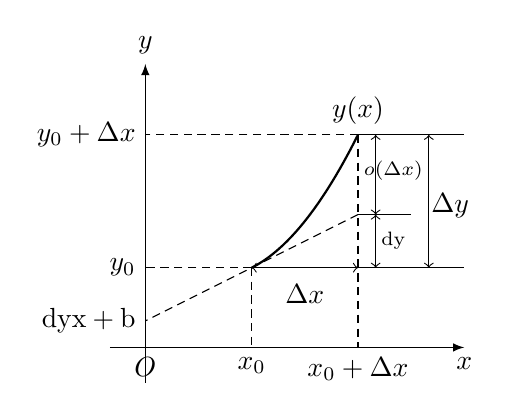
\begin{tikzpicture}[scale=0.9]
    \draw[-latex](-0.5,0) -- (4.5,0) node[below]{$x$};
    \draw[-latex](0,-0.5) -- (0,4) node[above]{$y$};
    \draw[black, thick, domain=1.5:3] plot (\x,{pow(\x-1,2)/2+1}) node[above]{$y(x)$};
    \filldraw[black] (0,0) node[below]{$O$};
    \draw[black, densely dashed](1.5,1.125) -- (1.5,0) node[below]{$x_0$};
    \draw[black, densely dashed](1.5,1.125) -- (0,1.125) node[left]{$y_0$};
    \draw[black, densely dashed](3,3) -- (3,0) node[below]{$x_0+\Delta x$};
    \draw[black, densely dashed](3,3) -- (0,3) node[left]{$y_0+\Delta x$};
    \draw[black, densely dashed](3,1.875) -- (0,0.375) node[left]{$\rm{d}yx+b$};
    \draw[<->, black](1.5,1.125) -- (3,1.125);
    \draw[<->, black](4,1.125) -- (4,3);
    \draw[<->, black](3.25,1.125) -- (3.25,1.875);
    \draw[<->, black](3.25,3) -- (3.25,1.875);
    \draw[black](3,3) -- (4.5,3);
    \draw[black](3,1.125) -- (4.5,1.125);
    \draw[black](3,1.875) -- (3.75,1.875);
    \filldraw[black] (2.25,0.75) node{$\Delta x$};
    \filldraw[black] (4.3,2) node{$\Delta y$};
    \filldraw[black] (3.5,1.5) node{\scriptsize{$\rm{d}y$}};
    \filldraw[black] (3.5,2.5) node{\scriptsize{$o(\Delta x)$}};
\end{tikzpicture}

所以可微就是用简单线性取代复杂线性,如图用直线取替代曲线。

\section{导数与微分计算}
\subsection{四则运算}

若函数可导:

\begin{enumerate}
    \item 和差的导数或微分:$[u(x)\pm v(x)]'=u'(x)\pm v'(x)$,$\rm{d}[u(x)\pm v(x)]=\rm{d}u(x)\pm\rm{d}v(x)$。
    \item 积的导数或微分:$[u(x)v(x)]'=u'(x)v(x)+u(x)v'(x)$,$\rm{d}[u(x)v(x)]=u(x)\rm{d}v(x)+v(x)\rm{d}u(x)$,$[u(x)v(x)w(x)]'=u'(x)v(x)w(x)+u(x)v'(x)w(x)+u(x)v(x)+w'(x)$。
    \item 商的导数:$\left[\dfrac{u(x)}{v(x)}\right]'=\dfrac{u'(x)v(x)-u(x)v'(x)}{[v(x)]^2}$,$\rm{d}\left[\dfrac{u(x)}{v(x)}\right]=\dfrac{v(x)\rm{d}u(x)-u(x)\rm{d}v(x)}{[v(x)]^2}$,$v(x)\neq 0$。
    \item 复合函数的导数:链式求导法则$\dfrac{\rm{d}u}{\rm{d}x}=\dfrac{\rm{d}u}{\rm{d}y}\cdot\dfrac{\rm{d}y}{\rm{d}x}$。
\end{enumerate}

\subsection{分段函数的导数}

设$f(x)=\left\{
    \begin{array}{lcl}
        f_1(x), & & x\geqslant x_0 \\
        f_2(x), & & x<x_0 \\
    \end{array}
\right.$。

在分段点用定义:判断$f'_+(x_0)=\lim_{x\to x_0^+}\dfrac{f_1(x)-f(x_0)}{x-x_0}\overset{?}{=}\lim_{x\to x_0^-}\dfrac{f_2(x)-f(x_0)}{x-x_0}$。

非分段点使用导数公式求导:$x>x_0,f'(x)=f_1'(x),x<0,f'(x)=f_2'(x)$。

\subsection{复合函数的导数与微分形式不变性}

$u=g(x)$在$x$可导,$y=f(u)$在$u=g(x)$处可导,则$\{f[g(x)]\}'=f'[g(x)]g'(x)$,$\rm{d}\{f[g(x)]\}=f'[g(x)]g'(x)\rm{d}x$。

一阶微分形式不变性指:$\rm{d}f(\varsigma)=f'(\varsigma)\rm{d}\varsigma$,无论$\varsigma$是什么。(类似导数的链式求导法则)

\textbf{例题7:}设$f(x)=\Pi_{n=1}^{100}\left(\tan\dfrac{\pi x^a}{4}-n\right)$,则$f'(1)$为?

原式=$\left(\tan\dfrac{\pi x}{4}-1\right)\left(\tan\dfrac{\pi x^2}{4}-2\right)\cdots\left(\tan\dfrac{\pi x^100}{4}-100\right)$。

令$\left(\tan\dfrac{\pi x^2}{4}-2\right)\cdots\left(\tan\dfrac{\pi x^100}{4}-100\right)=g(x)$。

$\therefore f(x)=\left(\tan\dfrac{\pi x}{4}-1\right)\cdot g(x)$。

$\therefore f'(x)=\sec^2\dfrac{\pi x}{4}\cdot\dfrac{\pi}{4}\cdot g(x)+\left(\tan\dfrac{\pi x}{4}-1\right)\cdot g'(x)$。

$\therefore$根据导数的四则运算,需要导数的乘积为每一项求导乘以其他不求导项的和,而$\tan\dfrac{\pi x}{4}-1$当$x=1$时为0,只要它不求导,其他的项都必然是0,所以原式的后面的结果都是0。

$\therefore$

$
\begin{aligned}
    f'(1) & =f'(x)\vert_{x=1} \\
    & =\dfrac{\pi}{2}\cdot g(1)+0\cdot g'(x) \\
    & =\dfrac{\pi}{2}\cdot g(1) \\
    & =\dfrac{\pi}{2}(-1)(-2)\cdots(-99) \\
    & =-\dfrac{\pi}{2}\cdot 99!
\end{aligned}
$

\textbf{例题8:}设$y=e^{\sin(\ln x)}$,求$\rm{d}y$。

$\because y=e^{\sin(\ln x)} \therefore$

$
\begin{aligned}
    \rm{d}y &=\rm{d}e^{\sin(\ln x)} \\
    & =e^{\sin(\ln x)}\cdot\rm{d}(\sin(\ln x)) \\
    & =e^{\sin(\ln x)}\cdot\cos(\ln x)\cdot\rm{d}\ln x \\
    & =e^{\sin(\ln x)}\cdot\cos(\ln x)\cdot\dfrac{1}{x}\rm{d}x
\end{aligned}
$

\subsection{反函数导数}

\textcolor{aqua}{\textbf{定理:}}$y=f(x)$可导,且$f'(x)\neq 0$,则存在反函数$x=\varphi(y)$,且$\dfrac{\rm{d}x}{\rm{d}y}=\dfrac{1}{\dfrac{\rm{d}y}{\rm{d}x}}$,即$\varphi'(x)=\dfrac{1}{f'(x)}$。

$y=f(x)$可导,且$f'(x)\neq 0$就是指严格单调,而严格单调必有反函数。

\textbf{例题9:}求$y=\arcsin x,x\in(-1,1)$与$y=\arctan x$的导数。

首先反三角函数就是三角函数的反函数、

求$y=\arcsin x$,即$x=\sin y$。

$\therefore\dfrac{\rm{d}\arcsin x}{\rm{d}x}=\dfrac{1}{\dfrac{\rm{d}\sin y}{\rm{d}y}}=\dfrac{1}{\cos y}=\dfrac{1}{\sqrt{1-\sin^2y}}=\dfrac{1}{\sqrt{1-x^2}}$。

求$y=\arctan x$,就$x=\tan y$。

$\therefore\dfrac{\rm{d}\arctan x}{\rm{d}x}=\dfrac{1}{\dfrac{\rm{d}\tan y}{\rm{d}y}}=\dfrac{1}{\sec^2y}=\dfrac{1}{1+\tan^2y}=\dfrac{1}{1+x^2}$。

\subsection{参数方程函数导数}
\subsection{隐函数求导法}
\subsection{对数求导法}
\subsection{幂指函数求导法}
\subsection{高阶导数}
\subsubsection{归纳法}
\subsubsection{莱布尼茨公式}
\subsubsection{泰勒公式}
\subsection{变限积分求导公式}

必然会考。

已知更改区间限制的积分$s(x)=\int_{\varphi_1(x)}^{\varphi_2(x)}g(t)\rm{d}x$,$s'(x)=g[\varphi_2(x)]\cdot\varphi_2'(x)-g[\varphi_1(x)]\cdot\varphi_1'(x)$。

\subsection{基本求导公式}
\end{document}
